% ══════════════════════════════════════════════════════════════════════════════
%  CAPITOLO — ANALISI ESPLORATIVA DEI DATI
%  Etichette: ch:eda, sec:demo, sec:types, sec:temporal, sec:collection,
%             sec:intensity, sec:denominatore, sec:eda_summary
% ══════════════════════════════════════════════════════════════════════════════

\chapter{Analisi Esplorativa dei Dati}
\label{ch:eda}

L'analisi che segue è basata sul dataset finale del \cref{ch:data}:
\textbf{353\,671 donazioni} di \textbf{43\,299 donatori distinti}, 2009--2025,
raccolte presso i punti di prelievo del DIMT di Trieste e Gorizia.

Il capitolo persegue tre scopi: descrivere chi sono i donatori; mostrare come e
dove donano; ed evidenziare le tendenze temporali che motivano la struttura dei
modelli dei capitoli successivi. La \cref{sec:denominatore} aggiunge una quarta
domanda, che le prime tre non possono rispondere: quanto del movimento
osservato è comportamento e quanto è semplicemente demografia.

% ---------------------------------------------------------------
\section{Profilo demografico dei donatori}
\label{sec:demo}

La popolazione di donatori è composta da \textbf{26\,737 uomini (61{,}7\%)} e
\textbf{16\,562 donne (38{,}3\%)}, con un rapporto M/F di circa $1{,}61$
(\cref{fig:gender}). La prevalenza maschile è sostanziale ed è in linea con i
dati nazionali del Centro Nazionale Sangue~\cite{cns2020}. La minore presenza femminile è
coerente con le restrizioni cliniche: prima della menopausa le donne possono
donare sangue intero due volte l'anno anziché quattro, e non possono donare
durante le mestruazioni o la gravidanza~\cite{donneDonazione}.

\begin{figure}[H]
    \centering
    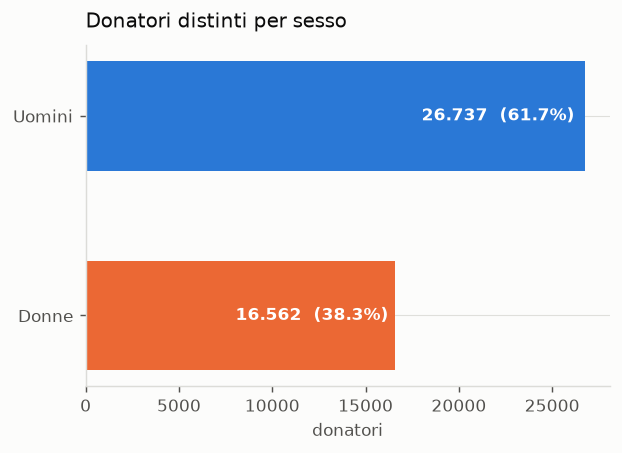
\includegraphics[width=0.55\linewidth]{img/fig_gender.png}
    \caption{Composizione per sesso dei donatori distinti, 2009--2025.}
    \label{fig:gender}
\end{figure}

L'età alla donazione (\cref{fig:age_hist}) ha media \textbf{42{,}4 anni},
mediana \textbf{44} e deviazione standard \textbf{12{,}0}, e va dai 18 anni
(minima età legale) ai 74; l'estremo superiore è coerente con la possibilità,
per i donatori periodici, di proseguire oltre i 65 anni sulla base della
valutazione clinica.

La forma non è però quella di una campana. Si riconoscono \textbf{due mode}:
un picco isolato a 18--19 anni --- l'effetto delle campagne di reclutamento
nelle scuole e della donazione al compimento della maggiore età --- seguito da
un avvallamento fra i 20 e i 30, e poi la moda principale intorno ai 47 anni,
su cui si concentra la massa della distribuzione. La fascia 30--55 rappresenta
la quota maggioritaria delle donazioni, mentre la 18--29 contribuisce con una
porzione minore --- un dato che la \cref{sec:denominatore} rileggerà, perché in
valore assoluto non dice quello che sembra dire.

\begin{figure}[H]
    \centering
    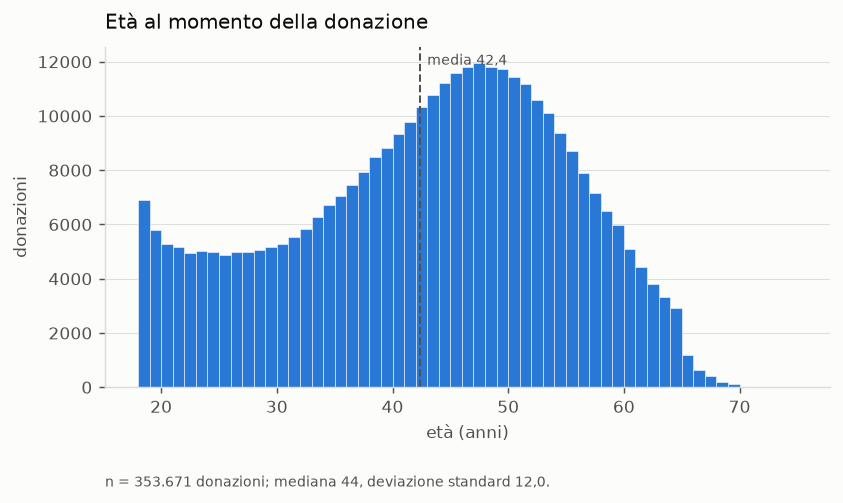
\includegraphics[width=0.85\linewidth]{img/fig_age_hist.png}
    \caption{Distribuzione dell'età al momento della donazione.}
    \label{fig:age_hist}
\end{figure}

Quanto all'adesione ad associazioni di volontariato (AVIS, ADSPEM, FIDAS e
altre), l'\textbf{81{,}7\%} dei donatori risulta associato in almeno una delle
proprie donazioni.

% ---------------------------------------------------------------
\section{Tipologie di donazione}
\label{sec:types}

Il dataset distingue dieci codici corrispondenti a sangue intero, plasmaferesi,
aferesi multicomponente e prelievi specialistici. Tre tipologie concentrano
il $99{,}7\%$ del volume (\cref{fig:types}): \textbf{sangue intero}
(267\,259 donazioni, $75{,}6\%$), \textbf{plasmaferesi} (75\,746, $21{,}4\%$) e
\textbf{aferesi piastrine + plasma} (9\,579, $2{,}7\%$). Le restanti sette
sommano circa lo $0{,}3\%$ (1\,087 donazioni) --- la più rara, la granulocitoaferesi, compare una
volta sola --- e nel dataset restano distinte; per semplicità, esse verranno accorpate in
un'unica categoria, "Altro", per le analisi successive.

\begin{figure}[H]
    \centering
    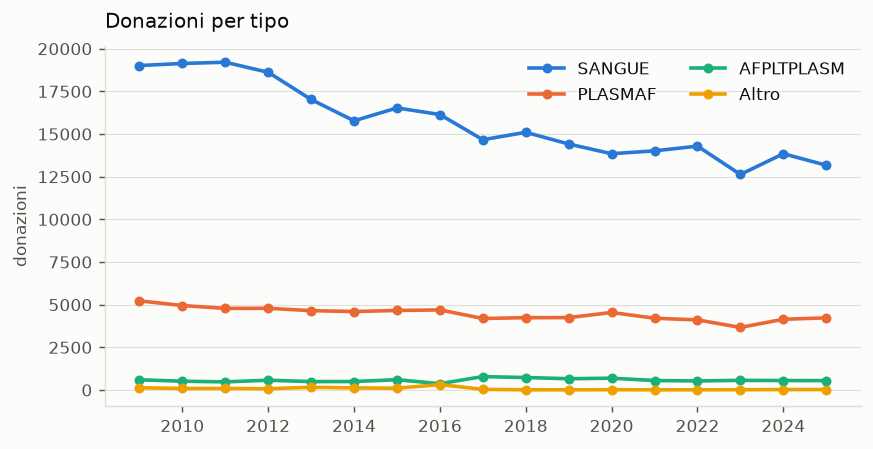
\includegraphics[width=0.80\linewidth]{img/fig_donation_types.png}
    \caption{Distribuzione delle donazioni per tipologia, 2009--2025.}
    \label{fig:types}
\end{figure}

\paragraph{Evoluzione della composizione nel tempo.}
La quota della plasmaferesi si mantiene sostanzialmente stabile
(\cref{fig:types_time}), con oscillazioni contenute in pochi punti percentuali
lungo tutto il periodo. La direzione è coerente con la spinta nazionale verso
l'autosufficienza~\cite{autosufficienza}, ma l'entità dell'effetto nel dataset
è modesta: la composizione per tipologia è la dimensione più immobile di tutto
il quadro descrittivo, e l'\cref{ch:forecast} la proietterà tale.

\begin{figure}[H]
    \centering
    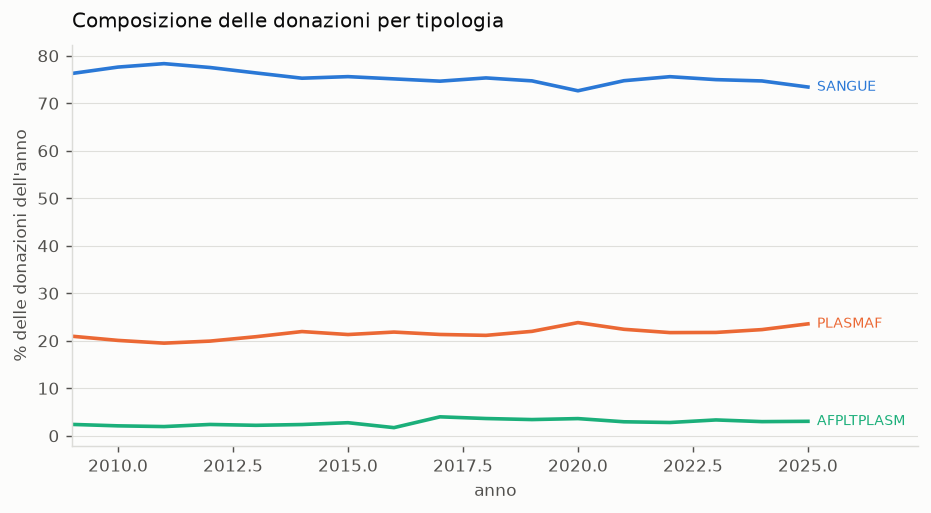
\includegraphics[width=0.95\linewidth]{img/fig_types_over_time.png}
    \caption{Composizione percentuale delle donazioni per tipologia, anno per
    anno.}
    \label{fig:types_time}
\end{figure}

% ---------------------------------------------------------------
\section{Tendenze temporali}
\label{sec:temporal}

\paragraph{Donazioni annuali.}
Il volume parte da circa \textbf{24\,900 donazioni} nel 2009, scende in modo
regolare fino a poco meno di 19\,300 nel 2019 e si assesta poi attorno alle
17--18 mila. Fra il primo e l'ultimo anno osservato la contrazione è del
\textbf{28{,}1\%} (\cref{fig:don_per_year}).

L'impatto della pandemia sul 2020 è stato \emph{più contenuto di quanto ci si
potesse attendere}: 19\,060 donazioni contro le 19\,289 del 2019, un calo
dell'$1{,}2\%$. Il dato è coerente con la posizione del Centro Nazionale
Sangue~\cite{cns2020} sulla tenuta del sistema trasfusionale italiano nei mesi
di lockdown, dovuta al
riconoscimento della donazione come attività essenziale e a un'ondata di
mobilitazione spontanea nelle prime settimane. Il 2023 segna il minimo della
serie (16\,840), con un parziale recupero nel biennio successivo.

\begin{figure}[H]
    \centering
    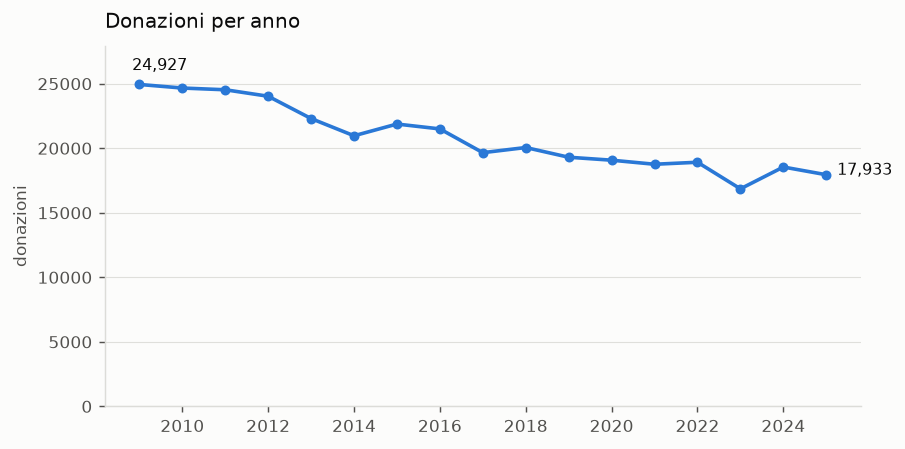
\includegraphics[width=0.95\linewidth]{img/fig_donations_per_year.png}
    \caption{Donazioni totali per anno, 2009--2025.}
    \label{fig:don_per_year}
\end{figure}

\paragraph{Nuovi donatori, e perché il 2009 non conta.}
Un secondo indicatore è il numero di donatori che entrano nel sistema ogni
anno. Qui però il primo anno della finestra non è un anno come gli altri: chi
compare per la prima volta nel 2009 non necessariamente \emph{inizia} nel 2009,
può semplicemente essere il primo anno in cui lo vediamo.

Il dato grezzo permette di distinguere i due casi, perché contiene la data di
inizio dell'attività donazionale (\cref{sec:decisioni}). Il risultato è netto:
dei 12\,957 donatori che nel 2009 risultano al primo evento osservato,
\textbf{il 65{,}9\% aveva già cominciato a donare prima}. Per loro la carriera
era iniziata, in mediana, nel 2002. Nel 2010 la quota di ``falsi ingressi'' è
ancora del $46{,}1\%$; dal 2011 in poi si stabilizza fra il 16 e il 29 per
cento, riflettendo il fatto che il campo non è sempre compilato.

L'avvio del sistema informativo nazionale SISTRA~\citep{sistra2007}, che le
Regioni dovevano recepire entro il 2008, spiega bene il fenomeno: donatori già
attivi da tempo ma non ancora tracciati elettronicamente compaiono come
``nuovi'' nel primo anno di rilevazione. La \cref{fig:new_donors} distingue le
due componenti; nel seguito \textbf{il 2009 è escluso dai confronti sui nuovi
ingressi}, e la flessione si misura dal 2010: da \textbf{1\,860 a 1\,149}
ingressi genuini fra il 2010 e il 2025, cioè $-38{,}2\%$, con un minimo di 960
nel 2021.

Qui è
considerato genuino chi non risulta \emph{esplicitamente} attivo prima, il che
include i donatori per cui la data di inizio manca del tutto: la domanda del
capitolo è quanti ingressi il sistema registra ogni anno, e togliere chi non ha
il campo compilato significherebbe togliere l'Isontino, per la ragione della
\cref{sec:decisioni}. Nel \cref{ch:retention}, in cui invece si segue una
coorte nel tempo, si adotta il criterio più restrittivo e si tiene solo chi ha una
data di inizio \emph{nota} e non anteriore all'anno del primo evento. Le due
serie divergono molto nei primi anni (nel 2010, 1\,860 contro 1\,360) e
convergono di fatto dal 2019 in poi, quando il campo è quasi sempre compilato.

\begin{figure}[H]
    \centering
    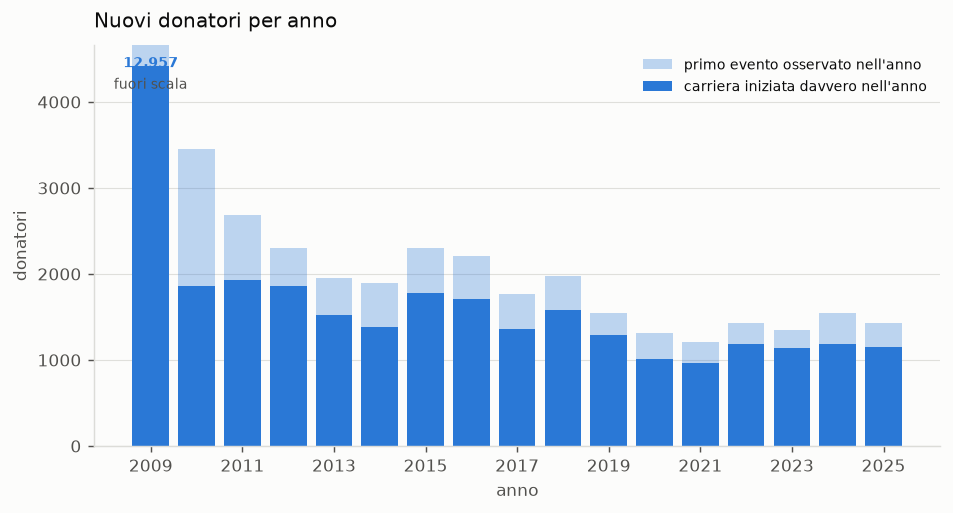
\includegraphics[width=0.95\linewidth]{img/fig_new_donors.png}
    \caption{Nuovi donatori per anno. La barra piena conta i soli donatori la
    cui attività comincia davvero in quell'anno; quella chiara aggiunge chi
    compare per la prima volta ma era già attivo prima.}
    \label{fig:new_donors}
\end{figure}

\paragraph{Stagionalità mensile.}
Sotto l'ipotesi di assenza di stagionalità ogni mese contribuirebbe all'$8{,}33\%$
del totale. Si osservano invece un picco primaverile (\textbf{marzo},
$9{,}24\%$) e autunnale (\textbf{ottobre}, $9{,}03\%$; settembre $8{,}80\%$),
un avvallamento estivo (\textbf{agosto}, $7{,}60\%$; luglio $7{,}86\%$) e uno
invernale meno marcato (\textbf{febbraio}, $7{,}95\%$), tipicamente associato
alle sospensioni per sindromi influenzali (\cref{fig:season}).

L'ampiezza è dell'ordine di $\pm 1$ punto percentuale: modesta ma sistematica.
Per evitare che il modello dell'\cref{ch:forecast} confonda questa variabilità
con il trend di lungo periodo, il mese vi entra come fattore esplicito.

\begin{figure}[H]
    \centering
    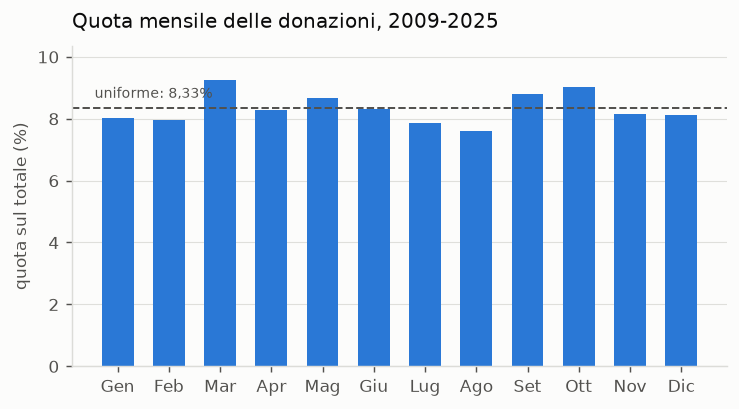
\includegraphics[width=0.95\linewidth]{img/fig_monthly_seasonality.png}
    \caption{Quota mensile delle donazioni sull'intero periodo. La linea
    tratteggiata indica la distribuzione uniforme attesa ($8{,}33\%$).}
    \label{fig:season}
\end{figure}

% ---------------------------------------------------------------
\section{Distribuzione geografica: punti di raccolta}
\label{sec:collection}

Il punto di raccolta non è registrato nei file del triennio 2021--2023, che hanno
un tracciato ridotto (\cref{sec:rawdata}): 54\,485 donazioni, il $15{,}4\%$ del
totale, ne sono prive, e le quote che seguono si riferiscono agli altri
quattordici anni. Sulle 299\,186 donazioni con punto di raccolta noto, l'ospedale
\textbf{Maggiore di Trieste} è di gran lunga il principale (152\,302
donazioni, $50{,}9\%$), seguito dalla \textbf{Sede di Gorizia} (49\,727,
$16{,}6\%$) e da \textbf{Monfalcone San Polo} (47\,601, $15{,}9\%$)
(\cref{fig:cp}).

Il dato ha una conseguenza sostanziale: \textbf{Gorizia non è un terzo polo
staccato, è appaiata a Monfalcone}, e i due siti isontini insieme valgono quasi
un terzo del sistema qui osservato. È l'effetto diretto della scelta discussa nella
\cref{sec:decisioni}: trattare la data di inizio attività come requisito di
ammissione avrebbe rimosso quasi la metà delle donazioni di Gorizia, che è
esattamente la sede in cui quel campo è meno compilato.

\begin{figure}[H]
    \centering
    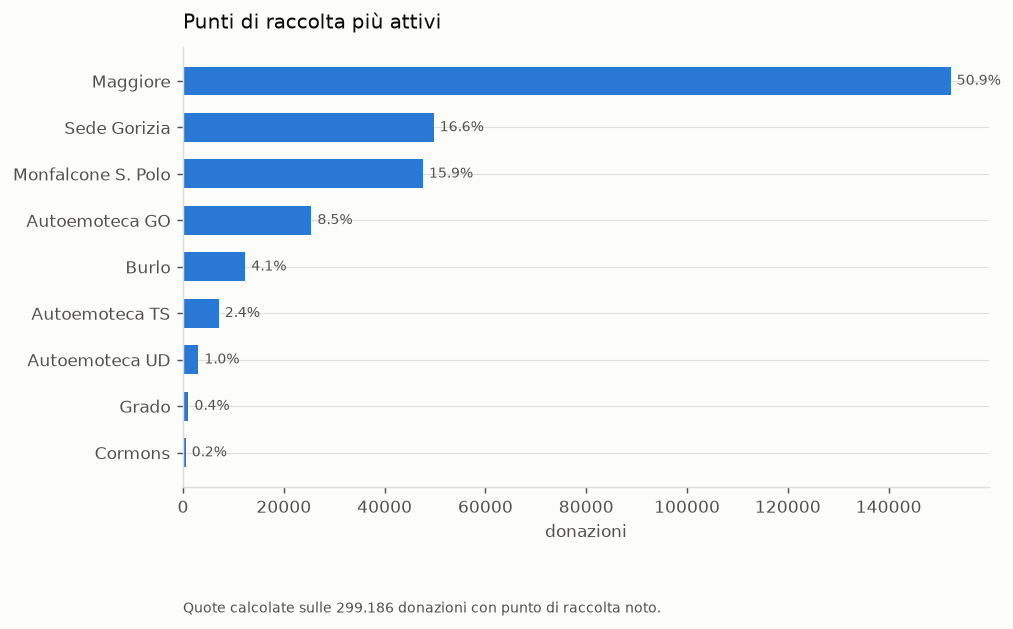
\includegraphics[width=0.95\linewidth]{img/fig_collection_points.png}
    \caption{Punti di raccolta più attivi, 2009--2025.}
    \label{fig:cp}
\end{figure}

% ---------------------------------------------------------------
\section{Intensità donazionale individuale}
\label{sec:intensity}

La distribuzione del numero di donazioni per donatore (\cref{fig:numdon}) è
fortemente asimmetrica a destra, con un notevole eccesso di donatori a una sola
donazione registrata e una coda lunga.

Va però osservato che questa figura misura la \emph{carriera}, non la
frequenza: somma donatori con due anni di attività e donatori con diciassette.
La misura pertinente per i modelli è il conteggio \emph{annuo}, sul panel
donatore-anno con gli anni a zero inclusi. Su quella misura la varianza è
$2{,}45$ volte la media: sovradispersione netta, che il \cref{ch:glm} dovrà
trattare esplicitamente. Sulla sola carriera dei donatori attivi il rapporto
scende a $1{,}23$, cioè quasi equidispersione --- lo stesso dato può quindi
sembrare o non sembrare sovradisperso a seconda dell'unità su cui lo si misura,
ed è una distinzione a cui il \cref{ch:glm} torna.

\begin{figure}[H]
    \centering
    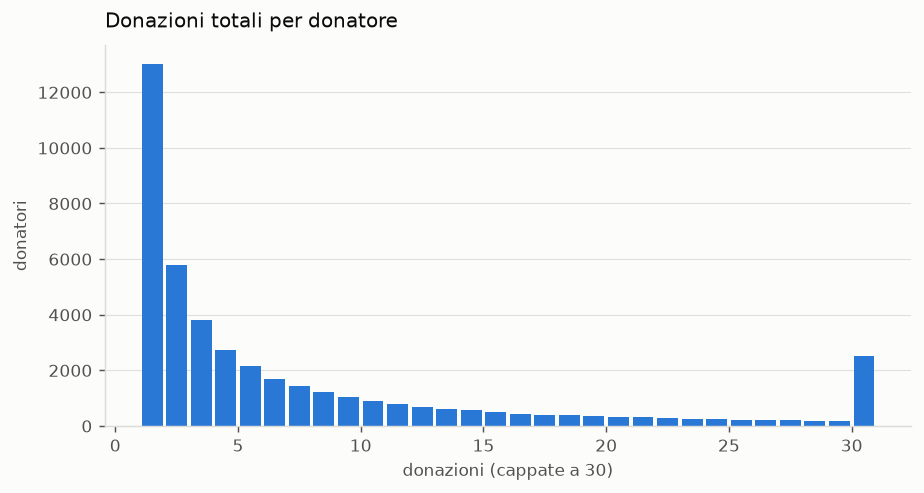
\includegraphics[width=0.85\linewidth]{img/fig_num_donations.png}
    \caption{Distribuzione del numero totale di donazioni per donatore (valori
    cappati a 30 per leggibilità).}
    \label{fig:numdon}
\end{figure}

Una seconda misura, meno vistosa ma più informativa, è il numero medio di
donazioni per donatore attivo in un anno. Resta in una banda di
\textbf{1{,}84--1{,}97 per tutti e diciassette gli anni}, senza tendenza: i
donatori attivi non donano oggi né più né meno spesso di quanto facessero nel
2009.

% ---------------------------------------------------------------
\section{Un denominatore: la popolazione residente}
\label{sec:denominatore}

Tutte le misure viste finora sono conteggi assoluti. Ma il territorio da cui
proviene il dato --- le province di Trieste e Gorizia --- perde abitanti e
invecchia: una parte del calo delle donazioni è meccanica, e finché non si
separano le due componenti l'affermazione ``il sistema è in erosione'' resta
indecidibile. La verifica è diretta: basta dividere per la popolazione in età
donabile.

\textbf{Il denominatore: popolazione di Trieste e Gorizia, non dell'intera
regione.} I dati di popolazione usati qui provengono da Eurostat al livello
NUTS-3 (\texttt{demo\_r\_pjanaggr3}, geo \texttt{ITH43} = Gorizia e
\texttt{ITH44} = Trieste~\cite{eurostatPjanaggr3NUTS3}), sommate fra le due
province: è la stessa area coperta dal DIMT e dalle donazioni al numeratore.
A questo livello di dettaglio geografico Eurostat pubblica solo tre fasce
ampie (\emph{under 15}, \emph{15--64}, \emph{65 e oltre}), non le fasce
quinquennali disponibili a livello regionale: si usa quindi la fascia
15--64 come proxy della popolazione in età donabile (18--64), leggermente più
ampia di quella esatta, perché le classi 15--17 pesano poco sul totale.

\paragraph{Quasi tutto il calo non è demografia.}
La popolazione di Trieste e Gorizia di 15--64 anni passa da 233\,144 a
223\,959 abitanti fra il 2009 e il 2025 ($-3{,}9\%$). Poiché le donazioni
sono il prodotto di quante persone potrebbero donare per quanto spesso lo
fanno, in logaritmi la variazione totale è la somma esatta delle due
componenti, senza residuo (\cref{tab:decomposizione}).

\begin{table}[ht]
\centering
\caption{Scomposizione del calo delle donazioni fra il 2009 e il 2025.}
\label{tab:decomposizione}
\begin{tabular}{@{}lrr@{}}
\toprule
\textbf{Componente} & \textbf{Variazione} & \textbf{Quota del calo} \\
\midrule
\textbf{Donazioni}                          & $-28{,}1\%$ & $100\%$ \\
\quad di cui: popolazione 15--64 (TS+GO)    & $\phantom{0}-3{,}9\%$  & $12{,}2\%$ \\
\quad di cui: donazioni per 1.000 residenti & $-25{,}1\%$ & $\mathbf{87{,}8\%}$ \\
\bottomrule
\end{tabular}
\end{table}

La demografia spiega poco meno di un \textbf{ottavo} del calo ($12{,}2\%$).
Quasi tutto il resto è perdita di partecipazione vera: si passa da
\textbf{106{,}9 a 80{,}1 donazioni ogni mille residenti} di 15--64 anni
(\cref{fig:per_1000}). Per il lavoro è un risultato che rafforza: l'erosione
è reale e non è un artefatto demografico. Senza il denominatore, l'obiezione
opposta sarebbe legittima e senza risposta.

\begin{figure}[H]
    \centering
    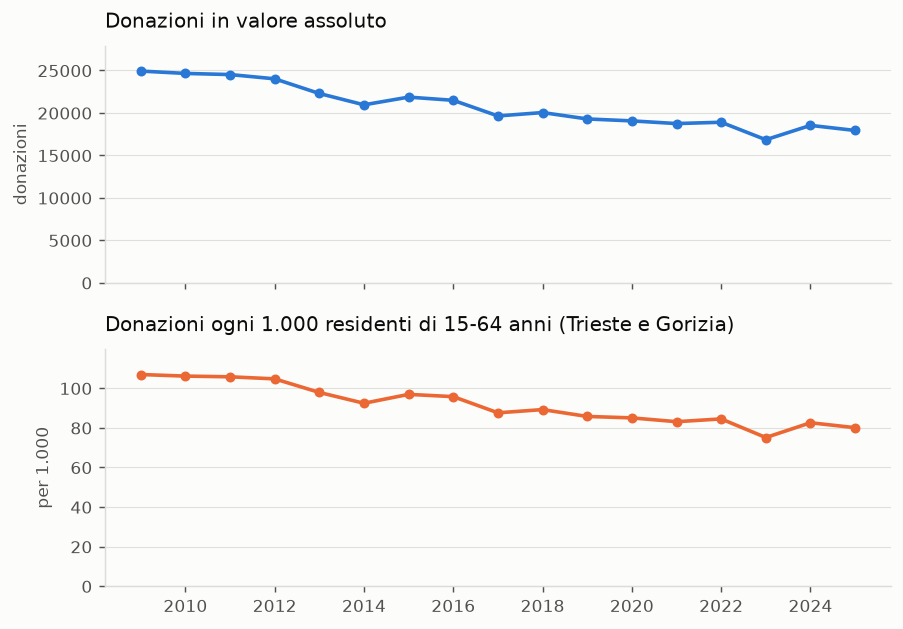
\includegraphics[width=0.9\linewidth]{img/fig_donazioni_per_1000.png}
    \caption{Donazioni in valore assoluto (sopra) e ogni mille residenti di
    15--64 anni di Trieste e Gorizia (sotto).}
    \label{fig:per_1000}
\end{figure}

\paragraph{Dove si è perso: non fra i giovani.}
Rapportando i donatori distinti alla popolazione della loro stessa fascia
d'età si ottiene il quadro della \cref{tab:tassi_eta}. Qui il denominatore
resta un limite dichiarato: a livello NUTS-3 Eurostat non pubblica fasce
quinquennali (\cref{sec:denominatore}), quindi questa tabella usa la
popolazione dell'intero Friuli Venezia Giulia
(\texttt{demo\_r\_pjangroup}~\cite{eurostatPjangroupNUTS2}) come proxy della
\emph{forma} del profilo per età, non del suo livello a Trieste e Gorizia. Il
quadro che ne risulta resta comunque controintuitivo rispetto a come la
questione viene di solito posta.

\begin{table}[ht]
\centering
\caption{Donatori distinti ogni mille residenti della stessa fascia d'età. Il
denominatore è la popolazione dell'intero Friuli Venezia Giulia (proxy della
forma del profilo, non del suo livello a Trieste e Gorizia).}
\label{tab:tassi_eta}
\begin{tabular}{@{}lrrr@{}}
\toprule
\textbf{Fascia} & \textbf{2009} & \textbf{2025} & \textbf{Variazione} \\
\midrule
\textbf{20--24} & $23{,}18$ & $\mathbf{19{,}21}$ & $-17{,}1\%$ \\
25--29 & $17{,}21$ & $17{,}64$ & $+2{,}5\%$ \\
30--34 & $18{,}75$ & $15{,}04$ & $-19{,}8\%$ \\
\textbf{35--39} & $21{,}14$ & $13{,}54$ & $\mathbf{-36{,}0\%}$ \\
\textbf{40--44} & $20{,}98$ & $12{,}37$ & $\mathbf{-41{,}0\%}$ \\
45--49 & $20{,}31$ & $14{,}72$ & $-27{,}5\%$ \\
50--54 & $16{,}58$ & $14{,}95$ & $\phantom{0}-9{,}8\%$ \\
55--59 & $12{,}21$ & $12{,}20$ & $\phantom{0}-0{,}1\%$ \\
60--64 & $\phantom{0}8{,}47$ & $\phantom{0}8{,}18$ & $\phantom{0}-3{,}4\%$ \\
65--69 & $\phantom{0}0{,}68$ & $\phantom{0}1{,}59$ & $+133{,}8\%$ \\
\bottomrule
\end{tabular}
\end{table}

Due letture, entrambe rilevanti per i capitoli successivi.

\textbf{Primo: a parità di popolazione, i giovani sono la fascia che dona di
più.} I 20--24enni hanno il tasso di partecipazione più alto in \emph{ogni}
anno osservato, 2025 compreso. Questo precisa i risultati ottenuti
nel \cref{ch:retention}: il problema dei giovani è che non
tornano a donare dopo le prime partecipazioni.

\textbf{Secondo: il crollo è a metà carriera.} Le fasce 35--44 perdono il
36--41\% del tasso di partecipazione, di gran lunga il calo maggiore, mentre le
fasce 55--64 sono sostanzialmente ferme e la 65--69 cresce (effetto
dell'estensione fino a 70 anni per i periodici). La \cref{fig:tassi_eta} lo
mostra in un colpo d'occhio: nel 2009 il profilo per età ha un ampio altopiano
fra i 35 e i 49 anni, nel 2025 quell'altopiano si è ristretto a un breve
pareggio fra i 45 e i 54 anni, e la curva scende in modo pressoché monotono
per tutte le fasce più giovani.

\begin{figure}[H]
    \centering
    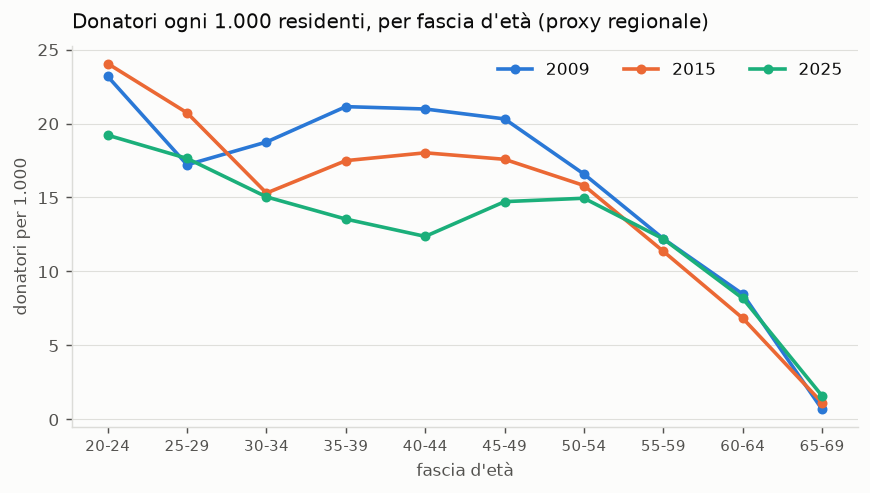
\includegraphics[width=0.9\linewidth]{img/fig_tassi_per_eta.png}
    \caption{Donatori ogni mille residenti per fascia d'età, in tre anni della
    serie.}
    \label{fig:tassi_eta}
\end{figure}

Il sistema, praticamente, ha perso i donatori di mezza età.
 Se questo sia un effetto di età o di coorte --- se cioè le
generazioni oggi trentacinquenni abbiano semplicemente sempre donato meno --- è
una domanda che i dati permettono di porre ma non, in questo lavoro, di
chiudere.

% ---------------------------------------------------------------
\section{Sintesi}
\label{sec:eda_summary}

\begin{enumerate}
    \item La popolazione di donatori è prevalentemente maschile ($61{,}7\%$) e
    di età media 42 anni: sesso ed età vanno controllati in tutti i modelli di
    frequenza.
    \item Il $99{,}7\%$ delle donazioni si concentra in tre tipologie, e la
    composizione fra queste è la dimensione più stabile del quadro.
    \item \textbf{Il volume annuale cala del $28{,}1\%$ fra il 2009 e il 2025},
    concentrando la flessione nella prima metà del periodo; i nuovi ingressi
    calano di più; e \textbf{l'intensità individuale non cambia}, restando fra
    $1{,}84$ e $1{,}97$ donazioni per donatore attivo. Il sistema non si è
    intensificato per compensare: si è ridotto e poi assestato su una base più
    piccola.
    \item \textbf{Solo un ottavo del calo è demografia} ($12{,}2\%$, sulla
    popolazione di Trieste e Gorizia), e la perdita di partecipazione si
    concentra nelle fasce 35--44, non fra i giovani, che restano la fascia
    con il tasso più alto. Resta un limite dichiarato sulla sola
    scomposizione \emph{per fascia d'età} (\cref{tab:tassi_eta}), che usa
    ancora la popolazione dell'intero FVG come proxy della forma del
    profilo, non essendo le fasce quinquennali disponibili a livello
    provinciale (\cref{sec:denominatore}).
    \item L'impatto del COVID-19 sul 2020 è stato modesto sulle donazioni
    ($-1{,}2\%$) ma marcato sui nuovi ingressi ($-21{,}5\%$): il modello aggregato
    deve poter assorbire uno shock puntuale.
    \item La stagionalità mensile è dell'ordine di $\pm 1$ punto percentuale,
    sistematica ma contenuta: va modellata come fattore per evitare confounding
    con il trend.
    \item La sovradispersione del conteggio dipende dall'unità di analisi:
    $2{,}45$ al grano donatore-anno con gli zeri, $1{,}23$ sui soli anni
    attivi. La scelta dell'unità nel \cref{ch:glm} non è quindi neutrale.
\end{enumerate}
